%This is chapter 3
%%=========================================
\chapter[Method]{Materials and methods}

%In this final chapter you should sum up what you have done and which results you have got. You should also discuss your findings, and give recommendations for further work.

%%=========================================

\section{Project Organization}
Do i need this?
The group consists of ...
Meetings ....


\section{Tools and libraries}
\subsection{JavaScript}

\subsection{Babel}
- Babel - ES6 needs to be transpiled to ES5 (Browser compatibility).
\subsection{npm}
Needed packages.. Published all packages to npm.. Most stabile compared to GitHubs new repo....

\subsection{Third party libraries}
Why did i use them???
list up like:
- xxx because ...
- xxx provides ...
Elaborate some on three.js - why is it good? (popularity)

\subsection{GitHub Actions}
Why? How did i use it? - For automation... - deeply integrated in GitHub.

\section{Working methodology}
\subsection{Scrum}
Even though this is a one man project, i have tried to adapt the scrum methodology.
...

\subsection{Requirements specification}
\subsubsection{Acceptance criteria}
Acceptance criteria - custom field in Jira.
Specially for the voxelization algorithm?

\subsection{GitFlow}
Why did i follow gitflow? Any changes to the usage?? Good for enforcing standards, automation etc..

\subsection{Semantic versioning}
All published modules are enforcing Semantic versioning. This ....

\section{three-voxel-loader}
\subsection{Loading data}
Used Three.js internal "Loader" -> Factory pattern -> Octree
- XML
- VOX
- BINVOX -> Separate repo!
- 3D array

\subsection{Visualization}
Traverse the octree -> Level Of Detail support -> BufferGeometry (Many  cubes)
Merged BufferGeometry => Better performance -> only one draw call.
\subsection{Debugging}
Developed an example -> later polished so you can find it on github...

\section{Voxelizer}
Short intro
\subsection{implementation}
\colorbox{RubineRed}{UML diagram of system here}

\subsection{Voxelization}
Currently, the only voxelization algorithm that is implemented is mainly based on raycasting.

\colorbox{RubineRed}{SKIP?:
Alternatively to raycasting, one could make use of color picking. This is in principle significantly quicker than normal raycasting since it is computed on the GPU. One could render a "heightmap" from each side of the 3D model. Each pixel in the heightmaps could then be looped over, mapping the pixel color back to the face's location in space, representing a filled voxel. Even though effective, it has a severe downside. No hidden or internal structures would be detected with this sort of system. Raycasting is therefore the obvious choise, even thoug it is CPU bound.
}

The raycasting is supplied by three.js library. The library provides a thoughourly tested and accurate raycasting solution. However, it itterates every face.. O(n).. Not good... The implementation of a three.js plugin were therefore used. it uses BVH to speed up the raycasting from O(n) to O(log n).

\subsubsection{Shell voxelization}
Asd

\subsubsection{Solid voxelization}
\colorbox{RubineRed}{Maybe more discussion or result related?}
The solid voxelisation, or filled voxelisation, is achieved by interpreting the first raycast intersect as the surface of the object. From this point will everything be considered "inside" the object. When a second intersect is detected, the state is changed to be "outside" the object. A new hit would indicate "inside", and so on. This works verry well with a watertight (\colorbox{RubineRed}{edges are manifolded?}) 3D model, as can be seen from figure \ref{fig:filling-non-watertight-model}. However, when trying to fill an object which is not watertight, this can result in severe inaccuracies. This can be seen in figure \ref{fig:filling-watertight-model}

\begin{figure}[h]
    \centering
    \begin{subfigure}[b]{0.45\textwidth}
        \centering
        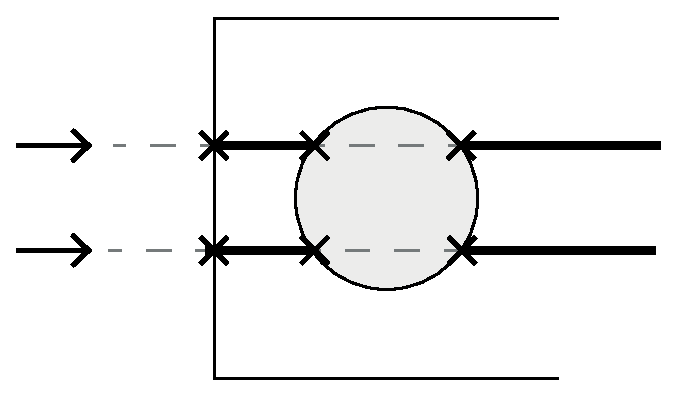
\includegraphics[width=\textwidth]{sections/methodology/figures/solid-non-watertight}
        \caption{Non-watertight 3D model cross section.}
        \label{fig:filling-non-watertight-model}
    \end{subfigure}
    \hfill
    \begin{subfigure}[b]{0.45\textwidth}
        \centering
        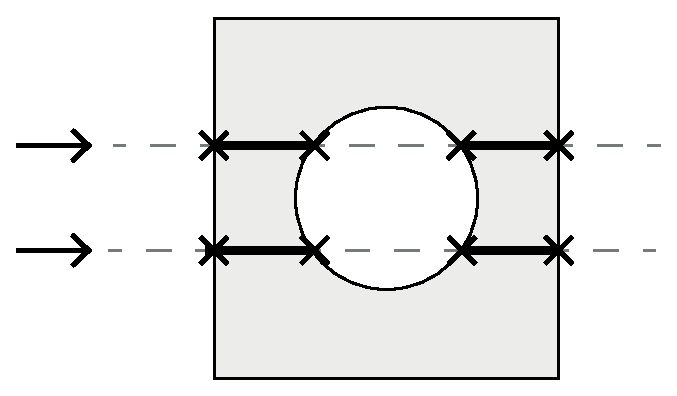
\includegraphics[width=\textwidth]{sections/methodology/figures/solid-watertight}
        \caption{Watertight 3D model cross section.}
        \label{fig:filling-watertight-model}
    \end{subfigure}
       \caption{Solid (voxelization) filling of 3D model cross section.}
       \label{fig:filling-3d-model}
\end{figure}


\subsection{Color system}
Reads object texture maps, extracts color etc...

\subsection{Loading}
The Voxelizer library/engine previously made use of a wrapper OBJ loader.
This support has been dropped in favor of the ES6 JS modules provided by three.js.

\subsection{Exporting}
- XML
- BINVOX (Separate repo)
- 3D array

\subsection{Debugging}
Developed an example -> later polished so you can find it on github...

\section{BINVOX}
A separate repo for building and parsing binvox files were constructed during refactoring of the voxelizer and the three-voxel-loader plugin....

\section{Voxelizer-Desktop}
\subsection{Electron}
\subsubsection{Auto updating}

\subsection{GUI}
... Sketches?? Wireframe diagrams of GUI etc...


\section{JSDoc Action}
Implementation in JS, not docker. Gives best possible speed, and cross compatibility (Win, linux and macos)
Can be used with any other action to upload to the desired service, for example GitHub pages.

\colorbox{RubineRed}{Diagram of implementation here}

\subsection{JSDoc}
Passes to cmd, loads configs, etc....

\subsection{Templates}
Support for templates. Downloads with the help of npm. Can be a github repository, npm package, etc...

\section{Automation}
\subsection{Workflows}
GitHub Actions...
Figure \ref{fig:cicd-pipelines} shows the continous integration and continous development pipelines. Describe how they work here....
\begin{figure}[h]
    \setlength{\abovecaptionskip}{25pt}
    \centering
    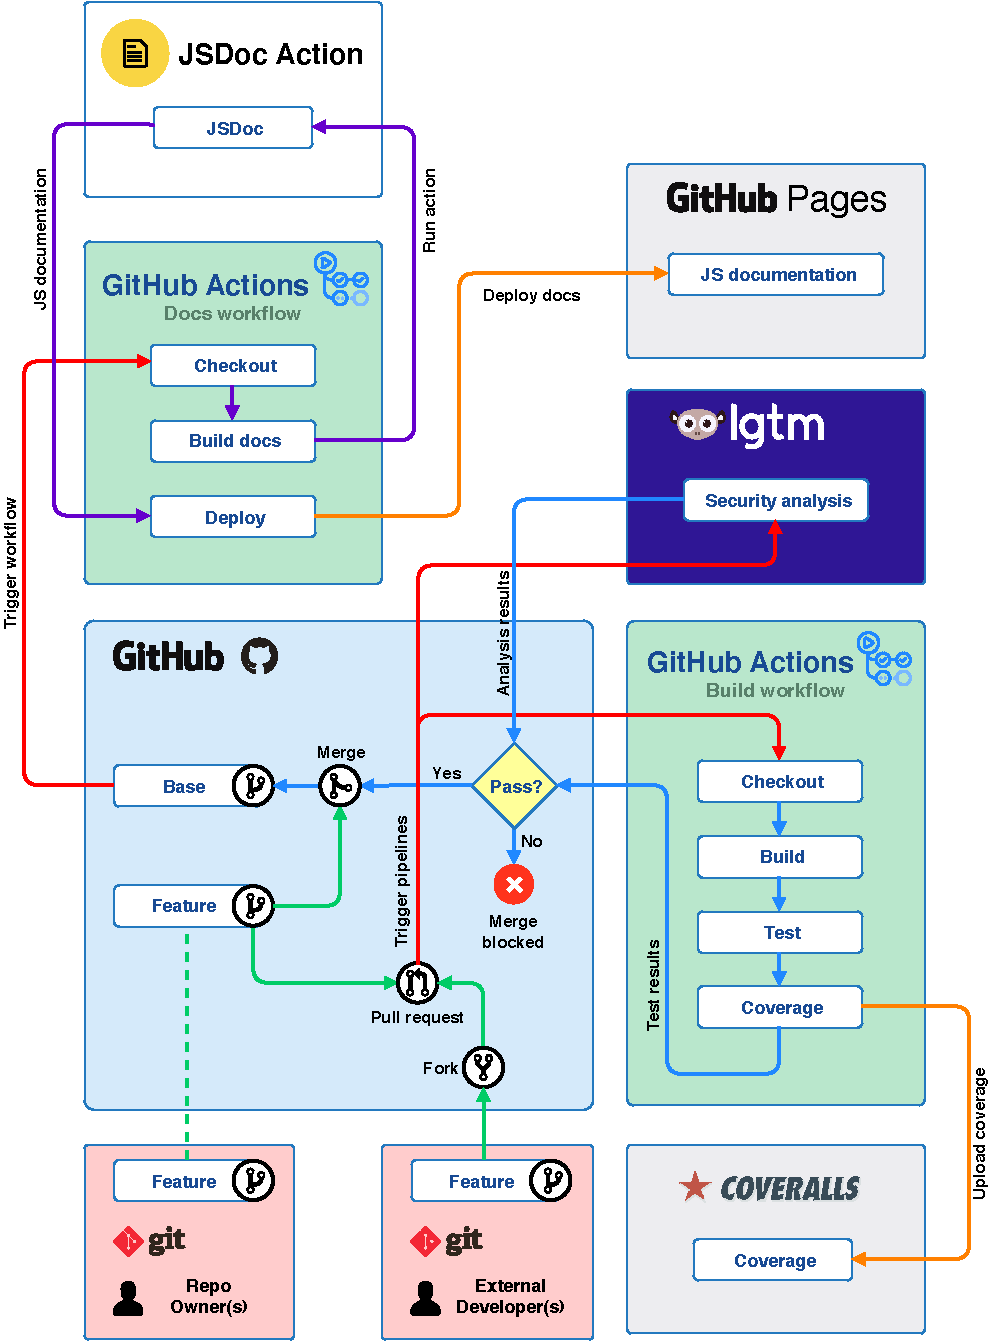
\includegraphics[page=1,scale=1]{sections/methodology/figures/pipelines.pdf}
    \caption{CI/CD pipelines}
    \label{fig:cicd-pipelines}
\end{figure}
\clearpage

And continue explaining here....
\subsubsection{Build}
\subsubsection{Test}
\subsubsection{Coverage}
Coveralls
\subsubsection{Security analysis}
LGTM
\subsubsection{Documentation generation}
JSDoc Action -> GitHub pages

\subsection{Release automation}

\subsubsection{Publish package}
See figure \ref{fig:release-automation}
\begin{figure}[h]
    \setlength{\abovecaptionskip}{25pt}
    \centering
    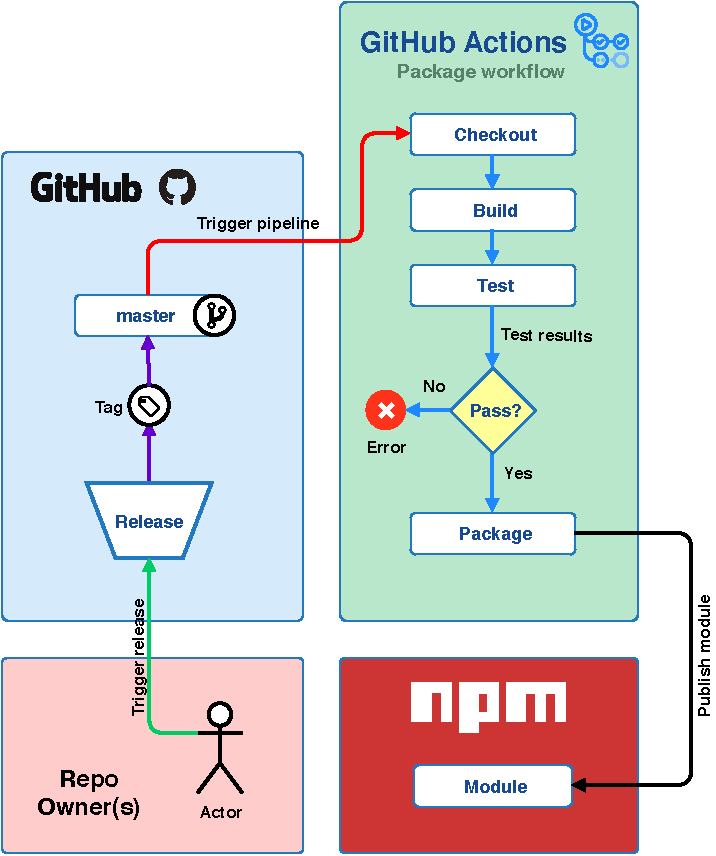
\includegraphics[page=1,scale=1]{sections/methodology/figures/package-release-automation.pdf}
    \caption{Automation of release publishing process.}
    \label{fig:release-automation}
\end{figure}

\subsubsection{GitHub Action version tagging}
Auto major version tagging update
See figure \ref{fig:update-major-tag}

\begin{figure}[h]
    \setlength{\abovecaptionskip}{25pt}
    \centering
    \hspace*{-2cm}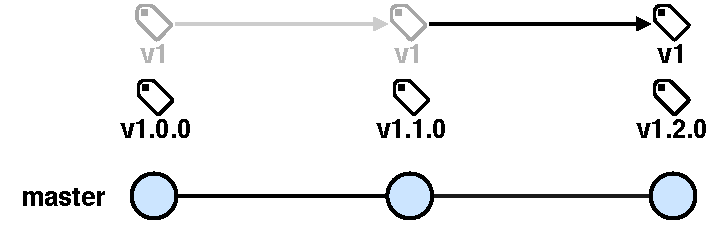
\includegraphics[page=1,scale=1]{sections/methodology/figures/update-major-tag.pdf}
    \caption{Automatic updating of major version tag.}
    \label{fig:update-major-tag}
\end{figure}

\subsection{Dependency updating}
Automated by Dependabot (accuired by GitHub).

\subsection{LaTeX generation}
Include how i have setup automation between my latex projects in order to generate thesis?

\section{file-existence-action}
During development of the workflows, it became apparent that i needed to be able to check if a file existed, and use this result in the following steps of the workflow.  This resulted in a relatively small GitHub action, named File Existence.

\section{file-reader-action}
During development of the workflows, it became apparent that i needed to be able to read the contents of a file, in order to check if it was empty and in that case, terminate the workflow. this resulted in a very small GitHub action, named File Reader.